\section{Minimality ed RFD Generation}
Le fasi di \emph{Minimality} e \emph{RFD Generation} sono le ultime due fasi dell'algoritmo. La fase di \emph{Minimality} prendendo come input gli \emph{insiemiC} dalla fase di \emph{Feasibility} generà sottoinsiemi di pattern minimali. L'output di tale fase sarà input della fase di \emph{RFD Generation} la quale genererà, da questi sottoinsiemi, le \textbf{RFD}. La fase di \emph{RFD Generation} non sarà oggetto di studio per questo lavoro di tesi.
\subsection{Nozioni preliminari}
Dalla fase di \emph{Feasibility} si otterranno per ogni RHS un certo numero di insiemi $C_i$ (con $i=1,...,m$) dove ogni $C_i$ sarà composto da un numero di pattern $P_j$ (con $j=1,...,h$) sull'insieme di attributi ($A_1$,...,$A_n$).
\subsection{Minimality}
L'obiettivo della fase di \emph{Minimality} è quello di determinare per ogni insieme $C_i$, generato come output dalla fase di \emph{Feasibility}, quei pattern che siano ammissibili e minimali. Diremo che un sotto-pattern $S_k$, definito come un insieme di attributi per i quali esistono pattern minimali, è ammissibile se quest'ultimo non domina rispetto a tutti gli altri nell'insieme $C_i$. Invece un sotto-pattern $S_k$ è minimale se esiste almeno un sotto-pattern di $S_k$ che non è ammissibile. Inizialmente l'algoritmo per ogni pattern $P_j$ calcola le differenze tra i valori di distanza di $P_j$ e i valori di distanza dei restanti pattern $P_y$, (con $y$ =1, 2, \ldots, h e $y \neq j$).
\begin{table}[H]
	\centering
	\begin{tabular}{ | l | l | l | l |}
		\hline
		& A & B & C \\
		\hline
		$T_{j1}$ & 1 & 5 & -4\\
		\hline
		. & . & . & .\\ 
		\hline
		. & . & . & . \\  
		\hline 
		$T_{jh}$ & 0 & 2 & -4\\ 
		\hline
	\end{tabular}
	\caption{Esempio di matrice per le distanze tra $P_j$ e $P_y$}
	\label{tab:table esempio}
\end{table}
Una volta calcolati tali valori e salvati in una matrice $M_{(h,n)}$ l'algoritmo, a partire dalla matrice appena creata, costruisce il \emph{Lattice}. Dato un generico insieme $A$ di $n$ elementi \{A,B,C\}, il \emph{Lattice} è una struttura dati ad albero che ha come radice l'insieme vuoto e come suoi figli gli attributi A,B,C. Iterativamente ad ogni livello $i$ dell'albero, si avrà tutte le possibili combinazioni di $n$ elementi di classe $i$.\\
\begin{center}
	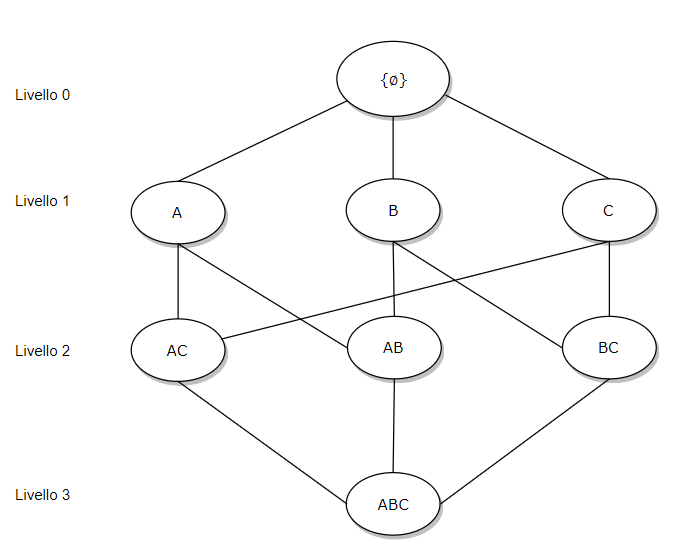
\includegraphics[scale = 0.60]{Immagini/Lattice.png}\\
\end{center}
Per ognuno dei nodi generati l'algoritmo effettua la verifica di minimalità. Definiamo $S_k$ ottimo se valgono le seguenti due proprietà:\\Con $|S_k| = 1$:\\$\bullet$ $\forall$ valore di $T_{jy} \in M_{(h,n)}$ $|$ $T_{jy} \leq 0$.\\Con $|S_k| > 1$:\\ $\bullet$ $\exists$ un valore di $T_{jy} \in M_{(h,n)}$ $|$ $T_{jy} < 0$, oppure $ \forall$  $T_{jy} \in M_{(h,n)}$, $T_{jy}= 0 $.\\ Affinché però si eviti di considerare super-set ammissibili di set minimali, applicheremo la tecnica del \emph{Pruning}. Il \emph{Pruning} è una tecnica che riduce le dimensioni degli alberi decisionali rimuovendo sezioni che non riconducono all'ottimo. Definiti tali concetti l'algoritmo, partendo dal livello 1, per ogni nodo dell'albero verifica due condizioni:\\1) Tutti i valori di $S_k$ sono positivi.\\2) Tutti i valori di $S_k$ sono negativi.\\Se si verifica uno solo dei due casi poc'anzi citati l'algoritmo elimina dal \emph{Lattice} tutti gli archi tra il nodo rappresentante $S_k$ e i suoi figli. L'output del \emph{Minimality} sarà dunque per ogni pattern $P_j$ i minimali $S_k$ per quel pattern.